\documentclass[11pt, a4paper]{article}
\usepackage{pdfpages}
\usepackage{parallel}
\usepackage[T2A]{fontenc}
\usepackage{ucs}
\usepackage[utf8x]{inputenc}
\usepackage[polish,english,russian]{babel}
\usepackage{hyperref}
\usepackage{rotating}
\usepackage[inner=2cm,top=1.8cm,outer=2cm,bottom=2.3cm,nohead]{geometry}
\usepackage{listings}
\usepackage{graphicx}
\usepackage{wrapfig}
\usepackage{longtable}
\usepackage{indentfirst}
\usepackage{array}
\usepackage{tikzsymbols}
\usepackage{soul}
\usepackage[ruled,vlined]{algorithm2e}
%\counterwithout{figure}{section} 

\usepackage{url}
\makeatletter
\g@addto@macro{\UrlBreaks}{\UrlOrds}
\makeatother

\newcolumntype{P}[1]{>{\raggedright\arraybackslash}p{#1}}
\frenchspacing
\usepackage{fixltx2e} %text sub- and superscripts
\usepackage{icomma} % коскі ў матэматычным рэжыме
\PreloadUnicodePage{4}

\newcommand{\longpage}{\enlargethispage{\baselineskip}}
\newcommand{\shortpage}{\enlargethispage{-\baselineskip}}

\def\switchlang#1{\expandafter\csname switchlang#1\endcsname}
\def\switchlangbe{
\let\saverefname=\refname%
\def\refname{Літаратура}%
\def\figurename{Іл.}%
}
\def\switchlangen{
\let\saverefname=\refname%
\def\refname{References}%
\def\figurename{Fig.}%
}
\def\switchlangru{
\let\saverefname=\refname%
\let\savefigurename=\figurename%
\def\refname{Литература}%
\def\figurename{Рис.}%
}

\hyphenation{admi-ni-stra-tive}
\hyphenation{ex-pe-ri-ence}
\hyphenation{fle-xi-bi-li-ty}
\hyphenation{Py-thon}
\hyphenation{ma-the-ma-ti-cal}
\hyphenation{re-ported}
\hyphenation{imp-le-menta-tions}
\hyphenation{pro-vides}
\hyphenation{en-gi-neering}
\hyphenation{com-pa-ti-bi-li-ty}
\hyphenation{im-pos-sible}
\hyphenation{desk-top}
\hyphenation{elec-tro-nic}
\hyphenation{com-pa-ny}
\hyphenation{de-ve-lop-ment}
\hyphenation{de-ve-loping}
\hyphenation{de-ve-lop}
\hyphenation{da-ta-ba-se}
\hyphenation{plat-forms}
\hyphenation{or-ga-ni-za-tion}
\hyphenation{pro-gramming}
\hyphenation{in-stru-ments}
\hyphenation{Li-nux}
\hyphenation{sour-ce}
\hyphenation{en-vi-ron-ment}
\hyphenation{Te-le-pathy}
\hyphenation{Li-nux-ov-ka}
\hyphenation{Open-BSD}
\hyphenation{Free-BSD}
\hyphenation{men-ti-on-ed}
\hyphenation{app-li-ca-tion}

\def\progref!#1!{\texttt{#1}}
\renewcommand{\arraystretch}{2} %Іначай формулы ў матрыцы зліпаюцца з лініямі
\usepackage{array}

\def\interview #1 (#2), #3, #4, #5\par{

\section[#1, #3, #4]{#1 -- #3, #4}
\def\qname{LVEE}
\def\aname{#1}
\def\q ##1\par{{\noindent \bf \qname: ##1 }\par}
\def\a{{\noindent \bf \aname: } \def\qname{L}\def\aname{#2}}
}

\def\interview* #1 (#2), #3, #4, #5\par{

\section*{#1\\{\small\rm #3, #4. #5}}
\ifx\ParallelWhichBox\undefined%
    \addcontentsline{toc}{section}{#1, #3, #4}%
\else%
\ifnum\ParallelWhichBox=0%
    \addcontentsline{toc}{section}{#1, #3, #4}%
\fi\fi%

\def\qname{LVEE}
\def\aname{#1}
\def\q ##1\par{{\noindent \bf \qname: ##1 }\par}
\def\a{{\noindent \bf \aname: } \def\qname{L}\def\aname{#2}}
}

\newcommand{\interviewfooter}[1]{
\vskip 1em
\noindent \textit{#1}
}

\switchlang{ru}
\begin{document}

\title{1986 "--- American Mouse}
\date{}
\maketitle
\selectlanguage{russian}
В 1986 году компания American Computer and Peripheral выпустила настольный компьютер American 286 на основе процессора i80286 \cite{adv}, комплектовавшийся манипулятором того же производителя под названием American Mouse (рис. \ref{fig:AmericanPic}). Цена устройства в отдельной продаже составляла \$125 \cite{review}.

\begin{figure}[h]
    \centering
    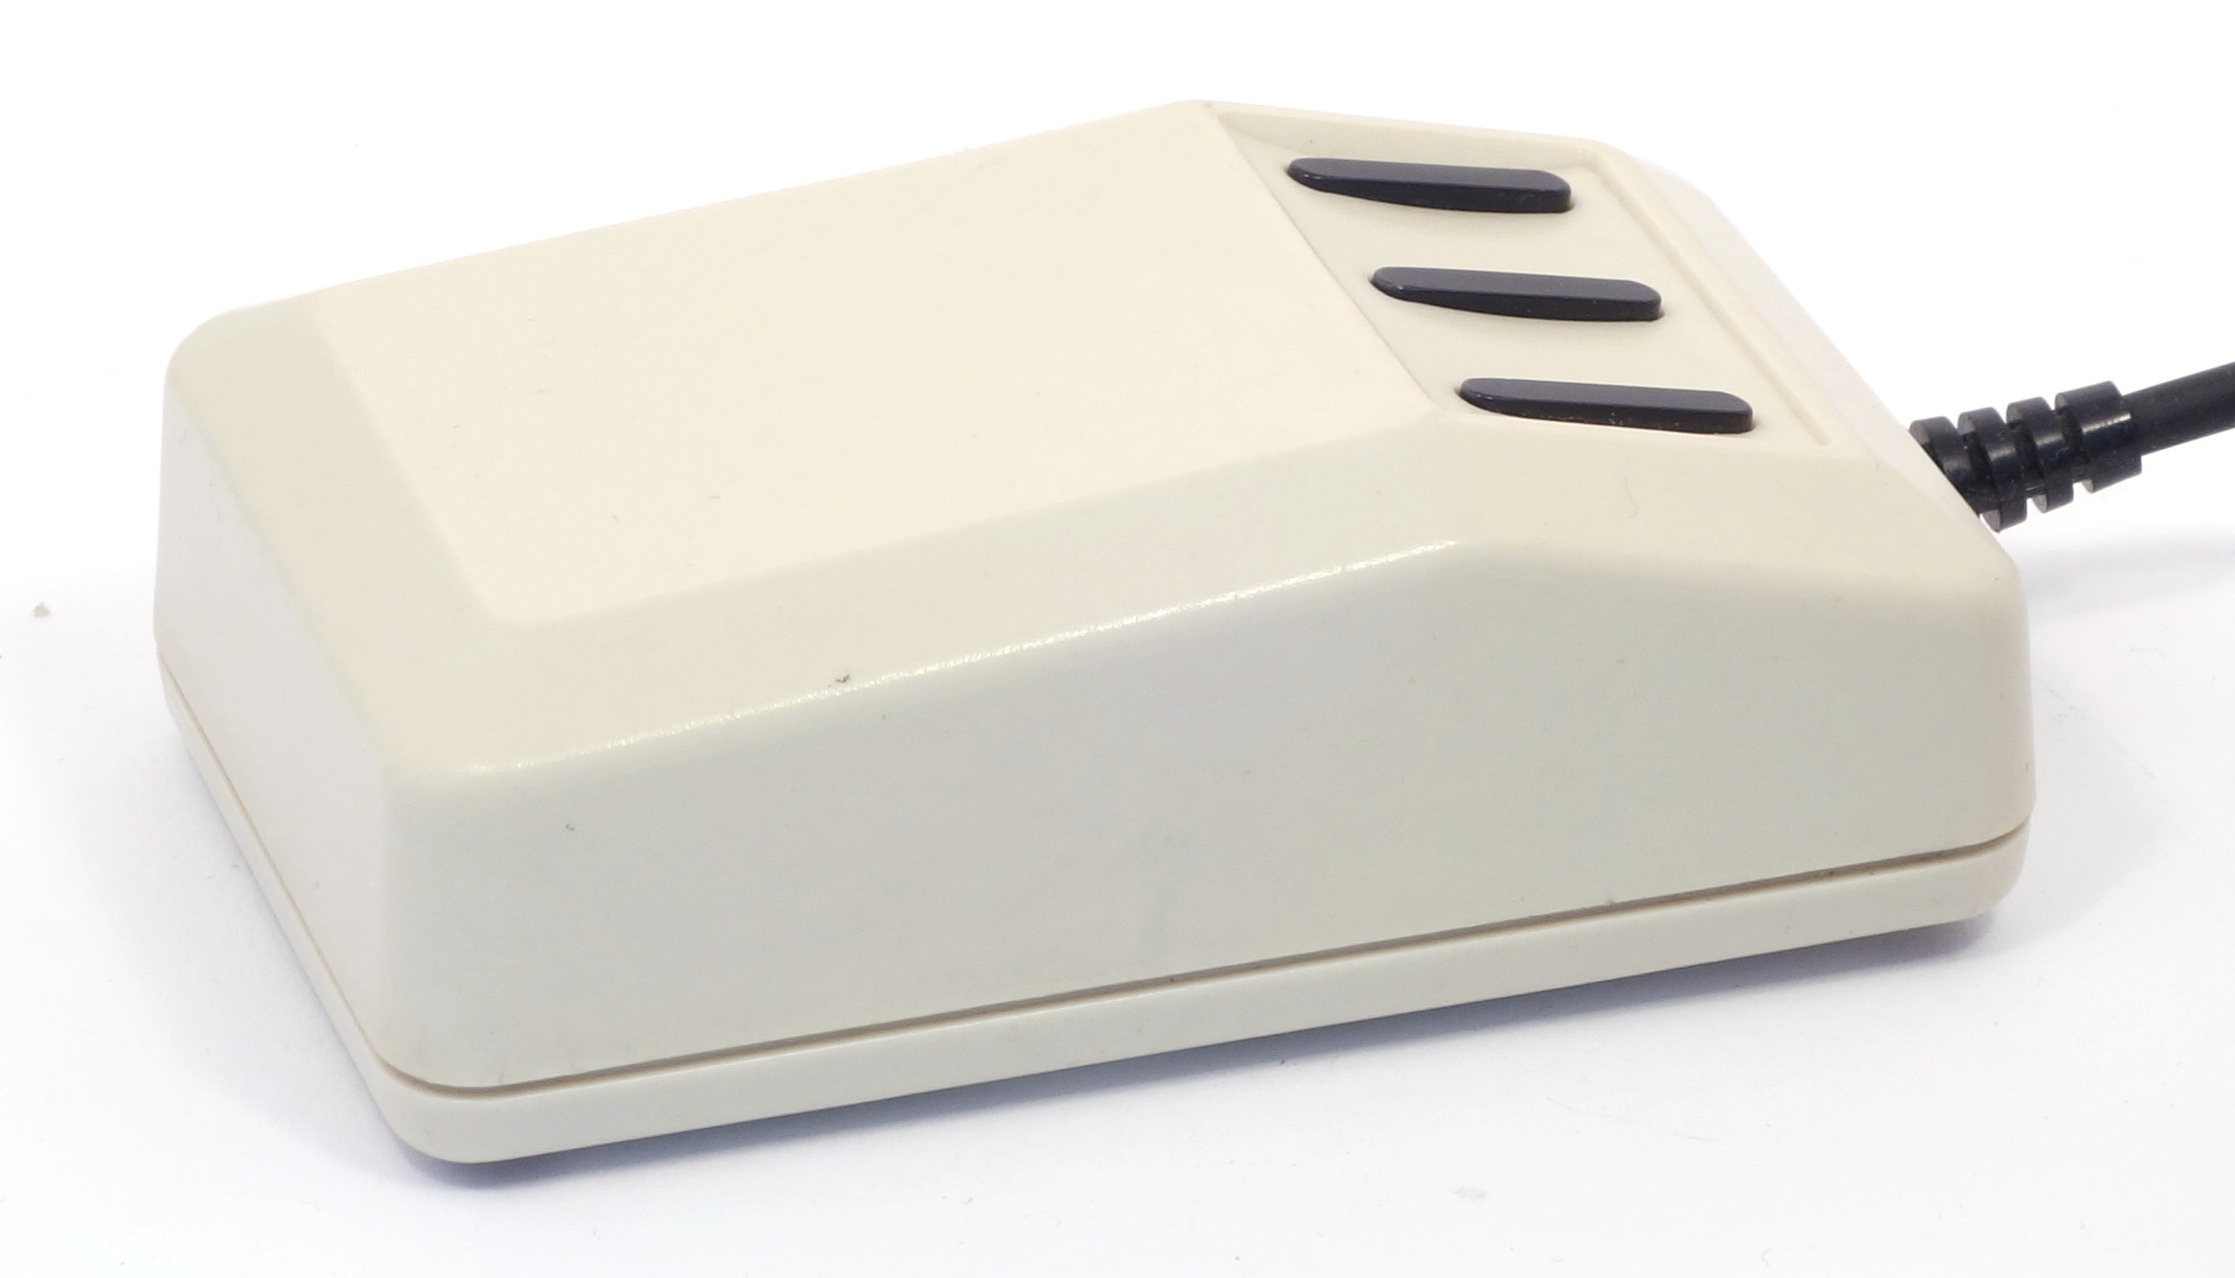
\includegraphics[scale=0.7]{1986_american_mouse/pic_30.jpg}
    \caption{American Mouse}
    \label{fig:AmericanPic}
\end{figure}

В углублении на слегка скошенной передней части крышки корпуса мыши расположены три феноменально узкие кнопки. Массивные переключатели, расположенные под кнопками, вынудили разработчиков применить асимметричное расположение кабеля мыши, проходящего между левой и средней кнопками (рис. \ref{AmericanTopAndBottom}). Нижняя сторона корпуса содержит съёмное кольцо для извлечения шара и очистки мыши. На корпусе отсутствуют какие-либо надписи или эмблемы.

\begin{figure}[h]
    \centering
    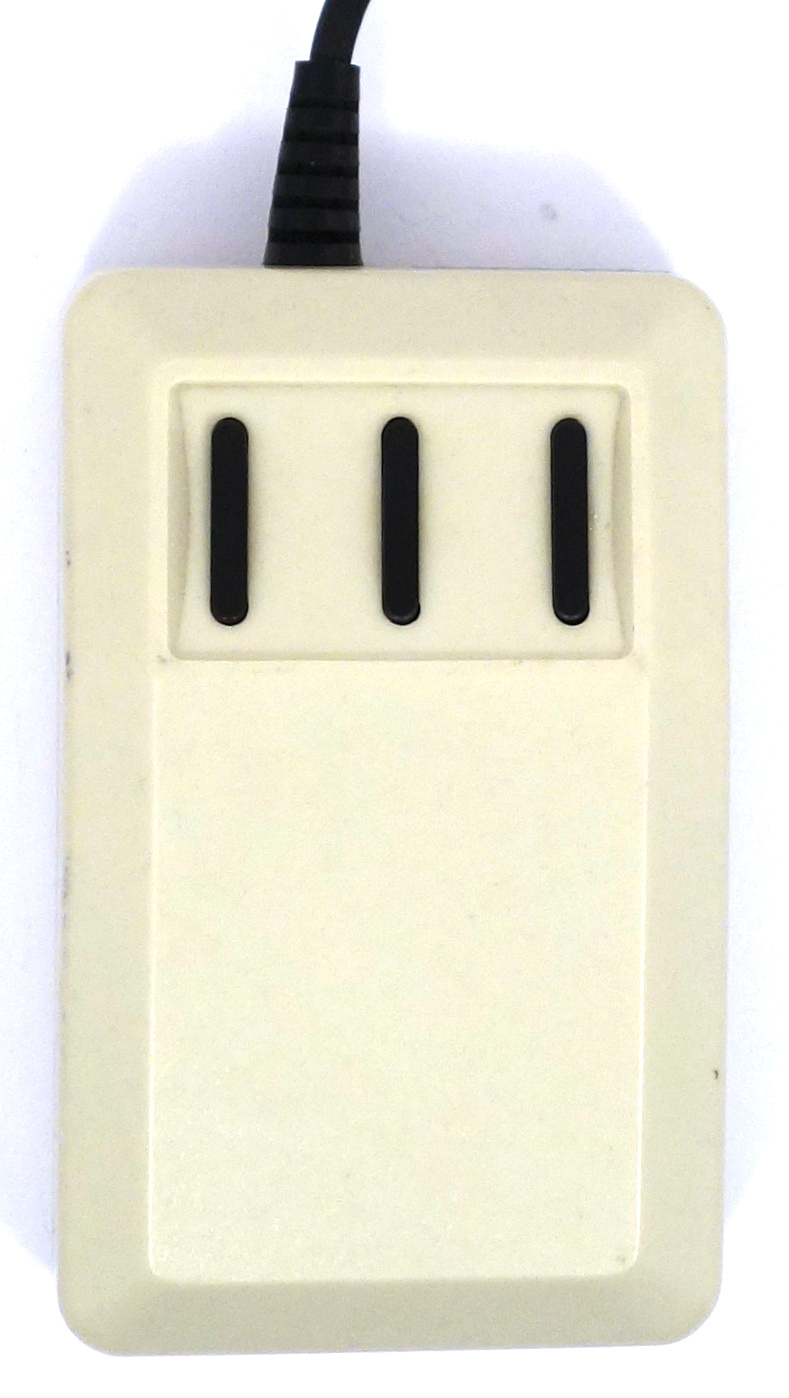
\includegraphics[scale=0.7]{1986_american_mouse/top_60.jpg}
    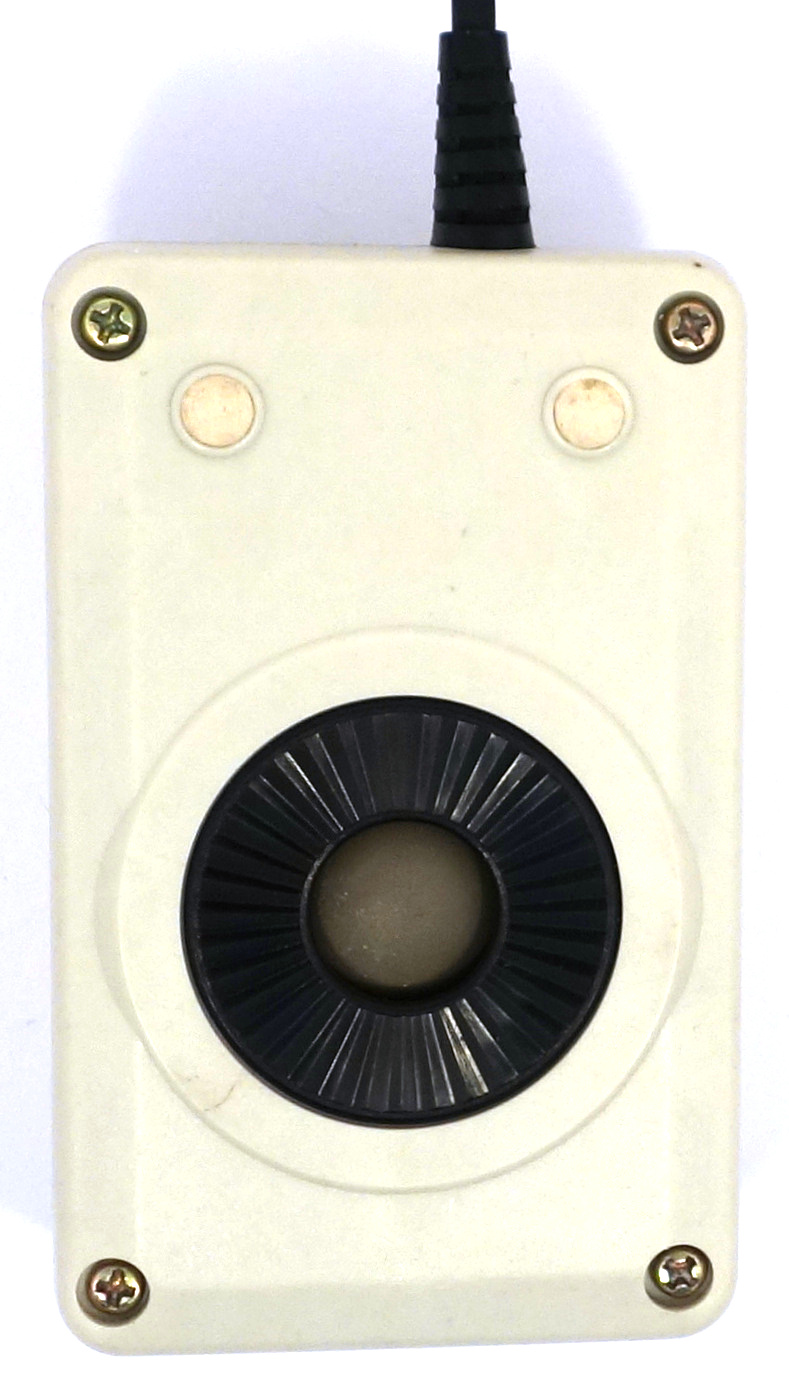
\includegraphics[scale=0.7]{1986_american_mouse/bottom_60.jpg}
    \caption{American Mouse, вид сверху и снизу}
    \label{AmericanTopAndBottom}
\end{figure}

В плане размера манипулятор представляет собой типичное для 80-х годов оптомеханическое устройство управления курсором (рис. \ref{fig:AmericanSize}).

\begin{figure}[h]
    \centering
    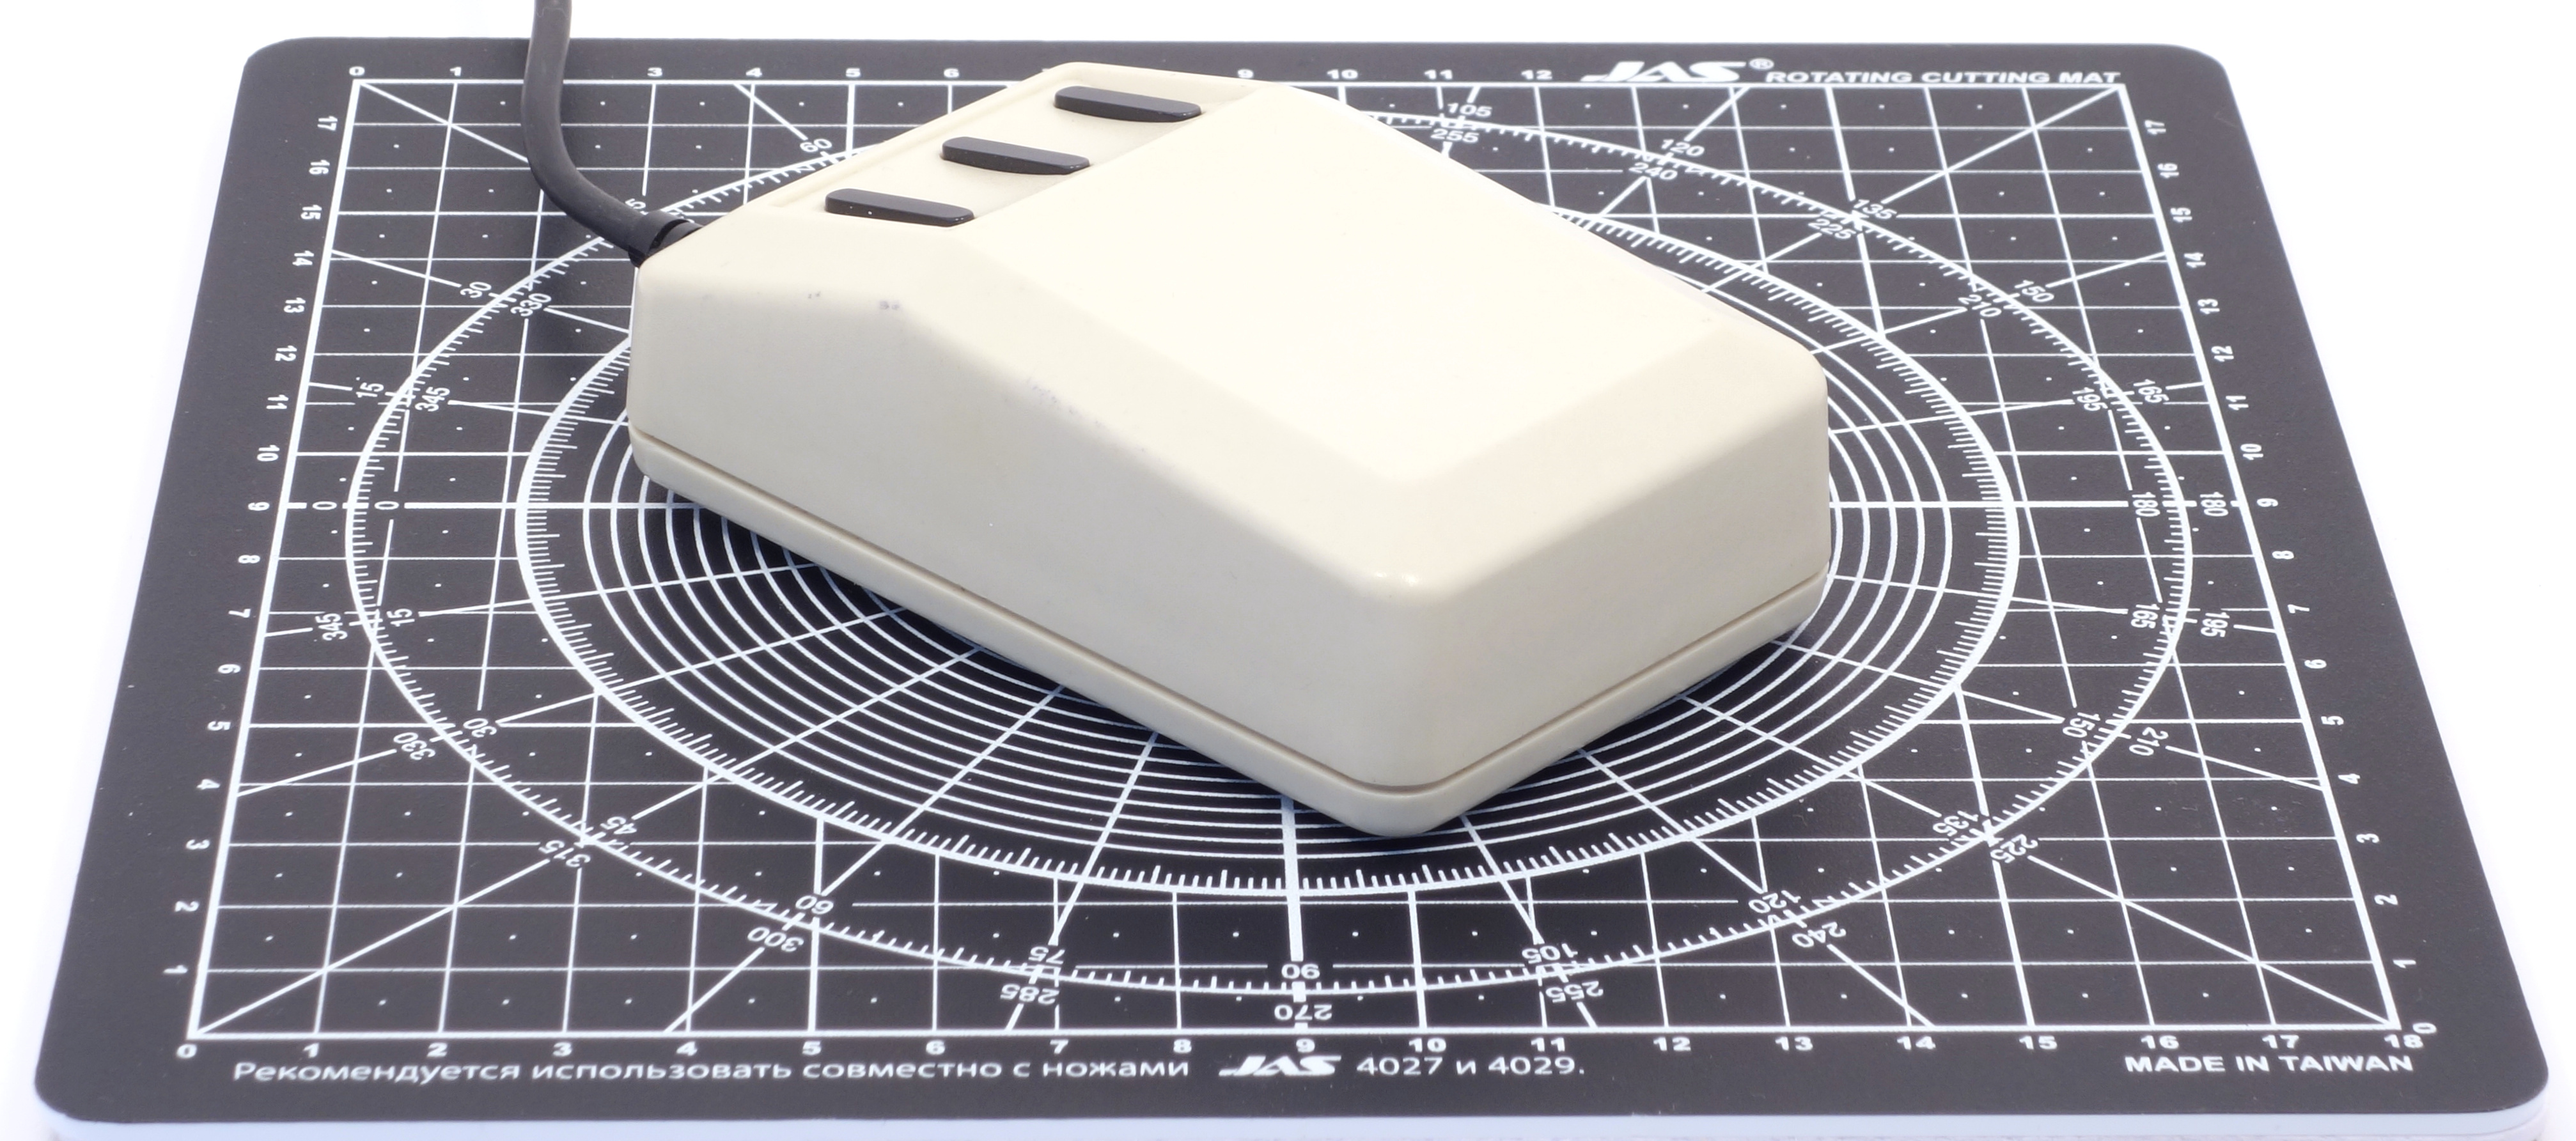
\includegraphics[scale=0.5]{1986_american_mouse/size_30.jpg}
    \caption{Изображение American Mouse на размерном коврике с шагом сетки 1~см}
    \label{fig:AmericanSize}
\end{figure}

Во внешнем виде American Mouse прослеживается индустриальный дизайн. При этом угловатый корпус оснастили скошенными гранями, чтобы обеспечить более комфортное расположение ладони; однако необходимость нажимать на чрезвычайно узкие кнопки, врезающиеся в подушечки пальцев, сводит на нет эргономические усилия разработчиков и позволяют причислить данный манипулятор к ряду устройств с наиболее сомнительным дизайном (рис. \ref{fig:AmericanHand}).

\begin{figure}[h]
    \centering
    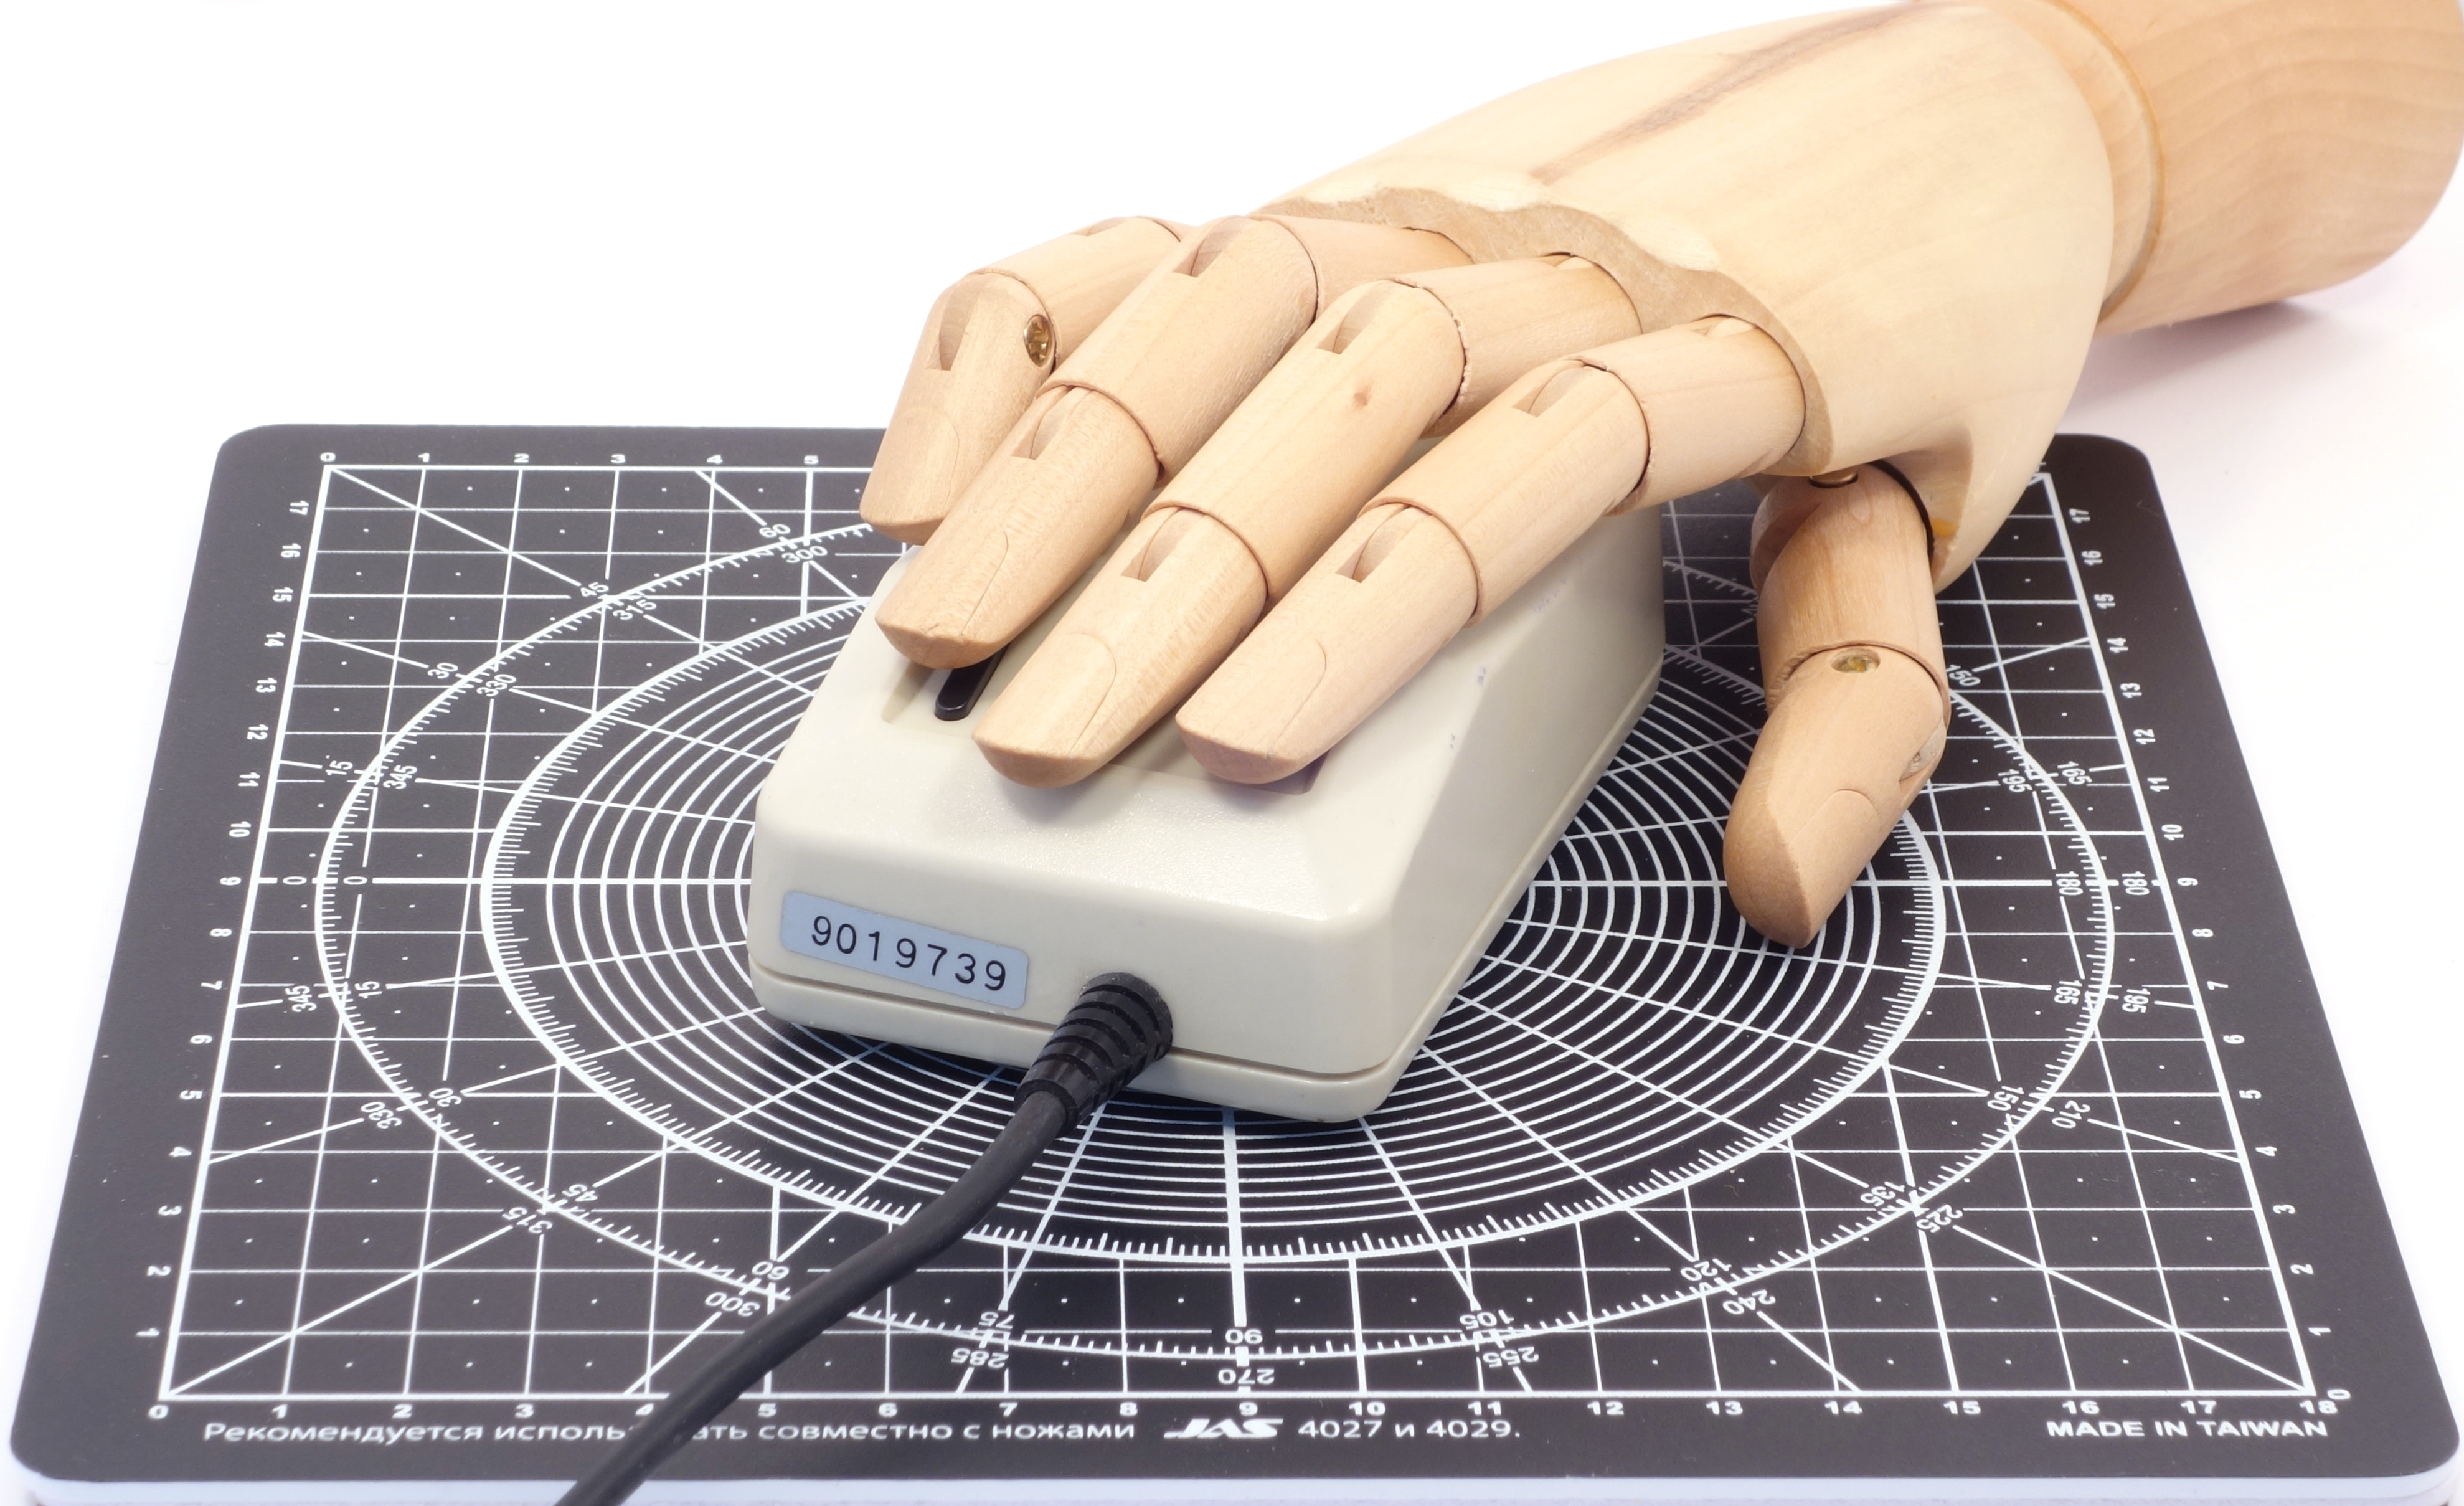
\includegraphics[scale=0.5]{1986_american_mouse/hand_30.jpg}
    \caption{American Mouse с моделью руки человека}
    \label{fig:AmericanHand}
\end{figure}

Americanl Mouse имеет разъём D-SUB и интерфейс подключения RS-232. Устройство работает по протоколу Mouse Systems, однако информация об этом отсутствует в сопроводительной брошюре, а драйвер данного протокола во время присутствия мыши на рынке можно было найти в основном в комплекте с оптическими мышами Mouse Systems, что ограничивало возможность использования American Mouse со сторонним программным обеспечением. В комплекте с мышью поставлялся единственный программный пакет "--- графический редактор Compu-Brush, представлявший собой ребрэндинг программы PC Paint.

\begin{figure}[h]
    \centering
    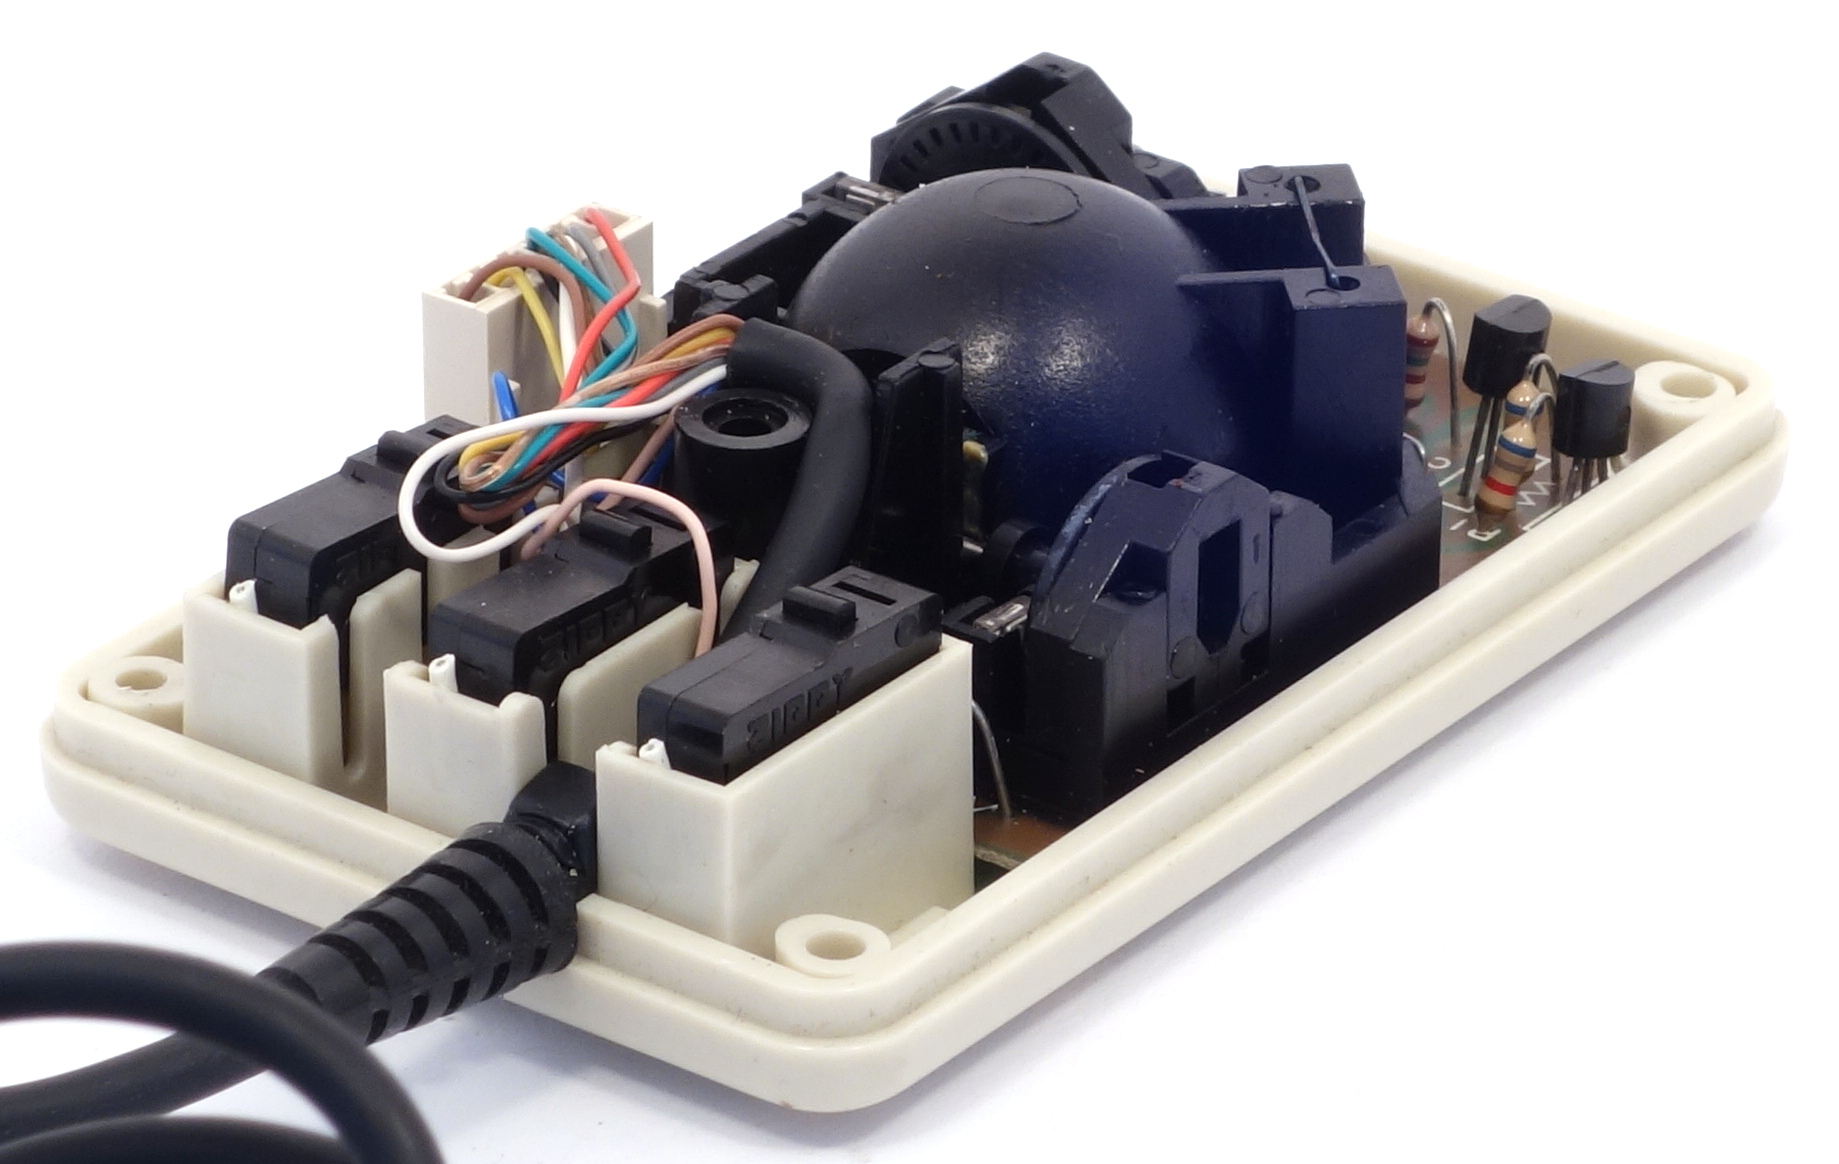
\includegraphics[scale=0.9]{1986_american_mouse/inside_60.jpg}
    \caption{American Mouse в разобранном виде}
    \label{fig:AmericanInside}
\end{figure}

В разобранном виде манипулятор показан на рис. \ref{fig:AmericanInside}, где можно увидеть достаточно стандартную конструкцию опто-механической мыши. Особенностью является плотное заполнение внутреннего пространства корпуса различными пластмассовыми деталями, которые отсутствуют в конструкциях практически пустотелых оптомеханических мышей более позднего периода.

\begin{thebibliography}{9}
\bibitem {adv} I love American (advertising). // PC MAGAZINE, V. 5, No. 18. October 1986, p. 157. \url{https://archive.org/details/PC-Mag-1986-10-28/page/n159}
\bibitem {review} Barr Ch. Mice for mainstream applications // PC MAGAZINE, V. 6, No. 14., August 1987, pp. 119 – 146 \url{https://archive.org/details/PC-Mag-1987-08-01/page/n121}
\end{thebibliography}
\end{document}
